%%%%%%%%%%%%%%%%%%%%%%%%%%%%%%%%%%%%%%%%%
% Stylish Article
% LaTeX Template
% Version 2.1 (1/10/15)
%
% This template has been downloaded from:
% http://www.LaTeXTemplates.com
%
% Original author:
% Mathias Legrand (legrand.mathias@gmail.com) 
% With extensive modifications by:
% Vel (vel@latextemplates.com)
% Final ACS by:
% Juan Barbosa
% License:
% CC BY-NC-SA 3.0 (http://creativecommons.org/licenses/by-nc-sa/3.0/)
%
%%%%%%%%%%%%%%%%%%%%%%%%%%%%%%%%%%%%%%%%%
\documentclass[fleqn,10pt]{SelfArx}
%\usepackage[superscript]{cite}
\usepackage{wrapfig}
%----------------------------------------------------------------------------------------
%	ARTICLE INFORMATION
%----------------------------------------------------------------------------------------

\JournalInfo{Laboratorio Avanzado, No. 2, 04/21/2017} % Journal information
\Archive{ }

\PaperTitle{S\'intesis inorg\'anicas} %
%\Keywords{Keyword1 --- Keyword2 --- Keyword3} % Keywords - if you don't want any simply remove all the text between the curly brackets
%\newcommand{\keywordname}{Keywords} % Defines the keywords heading name

%----------------------------------------------------------------------------------------
%	ABSTRACT
%----------------------------------------------------------------------------------------

\Abstract{
	\begin{wrapfigure}{r}{0.5\textwidth}
		\centering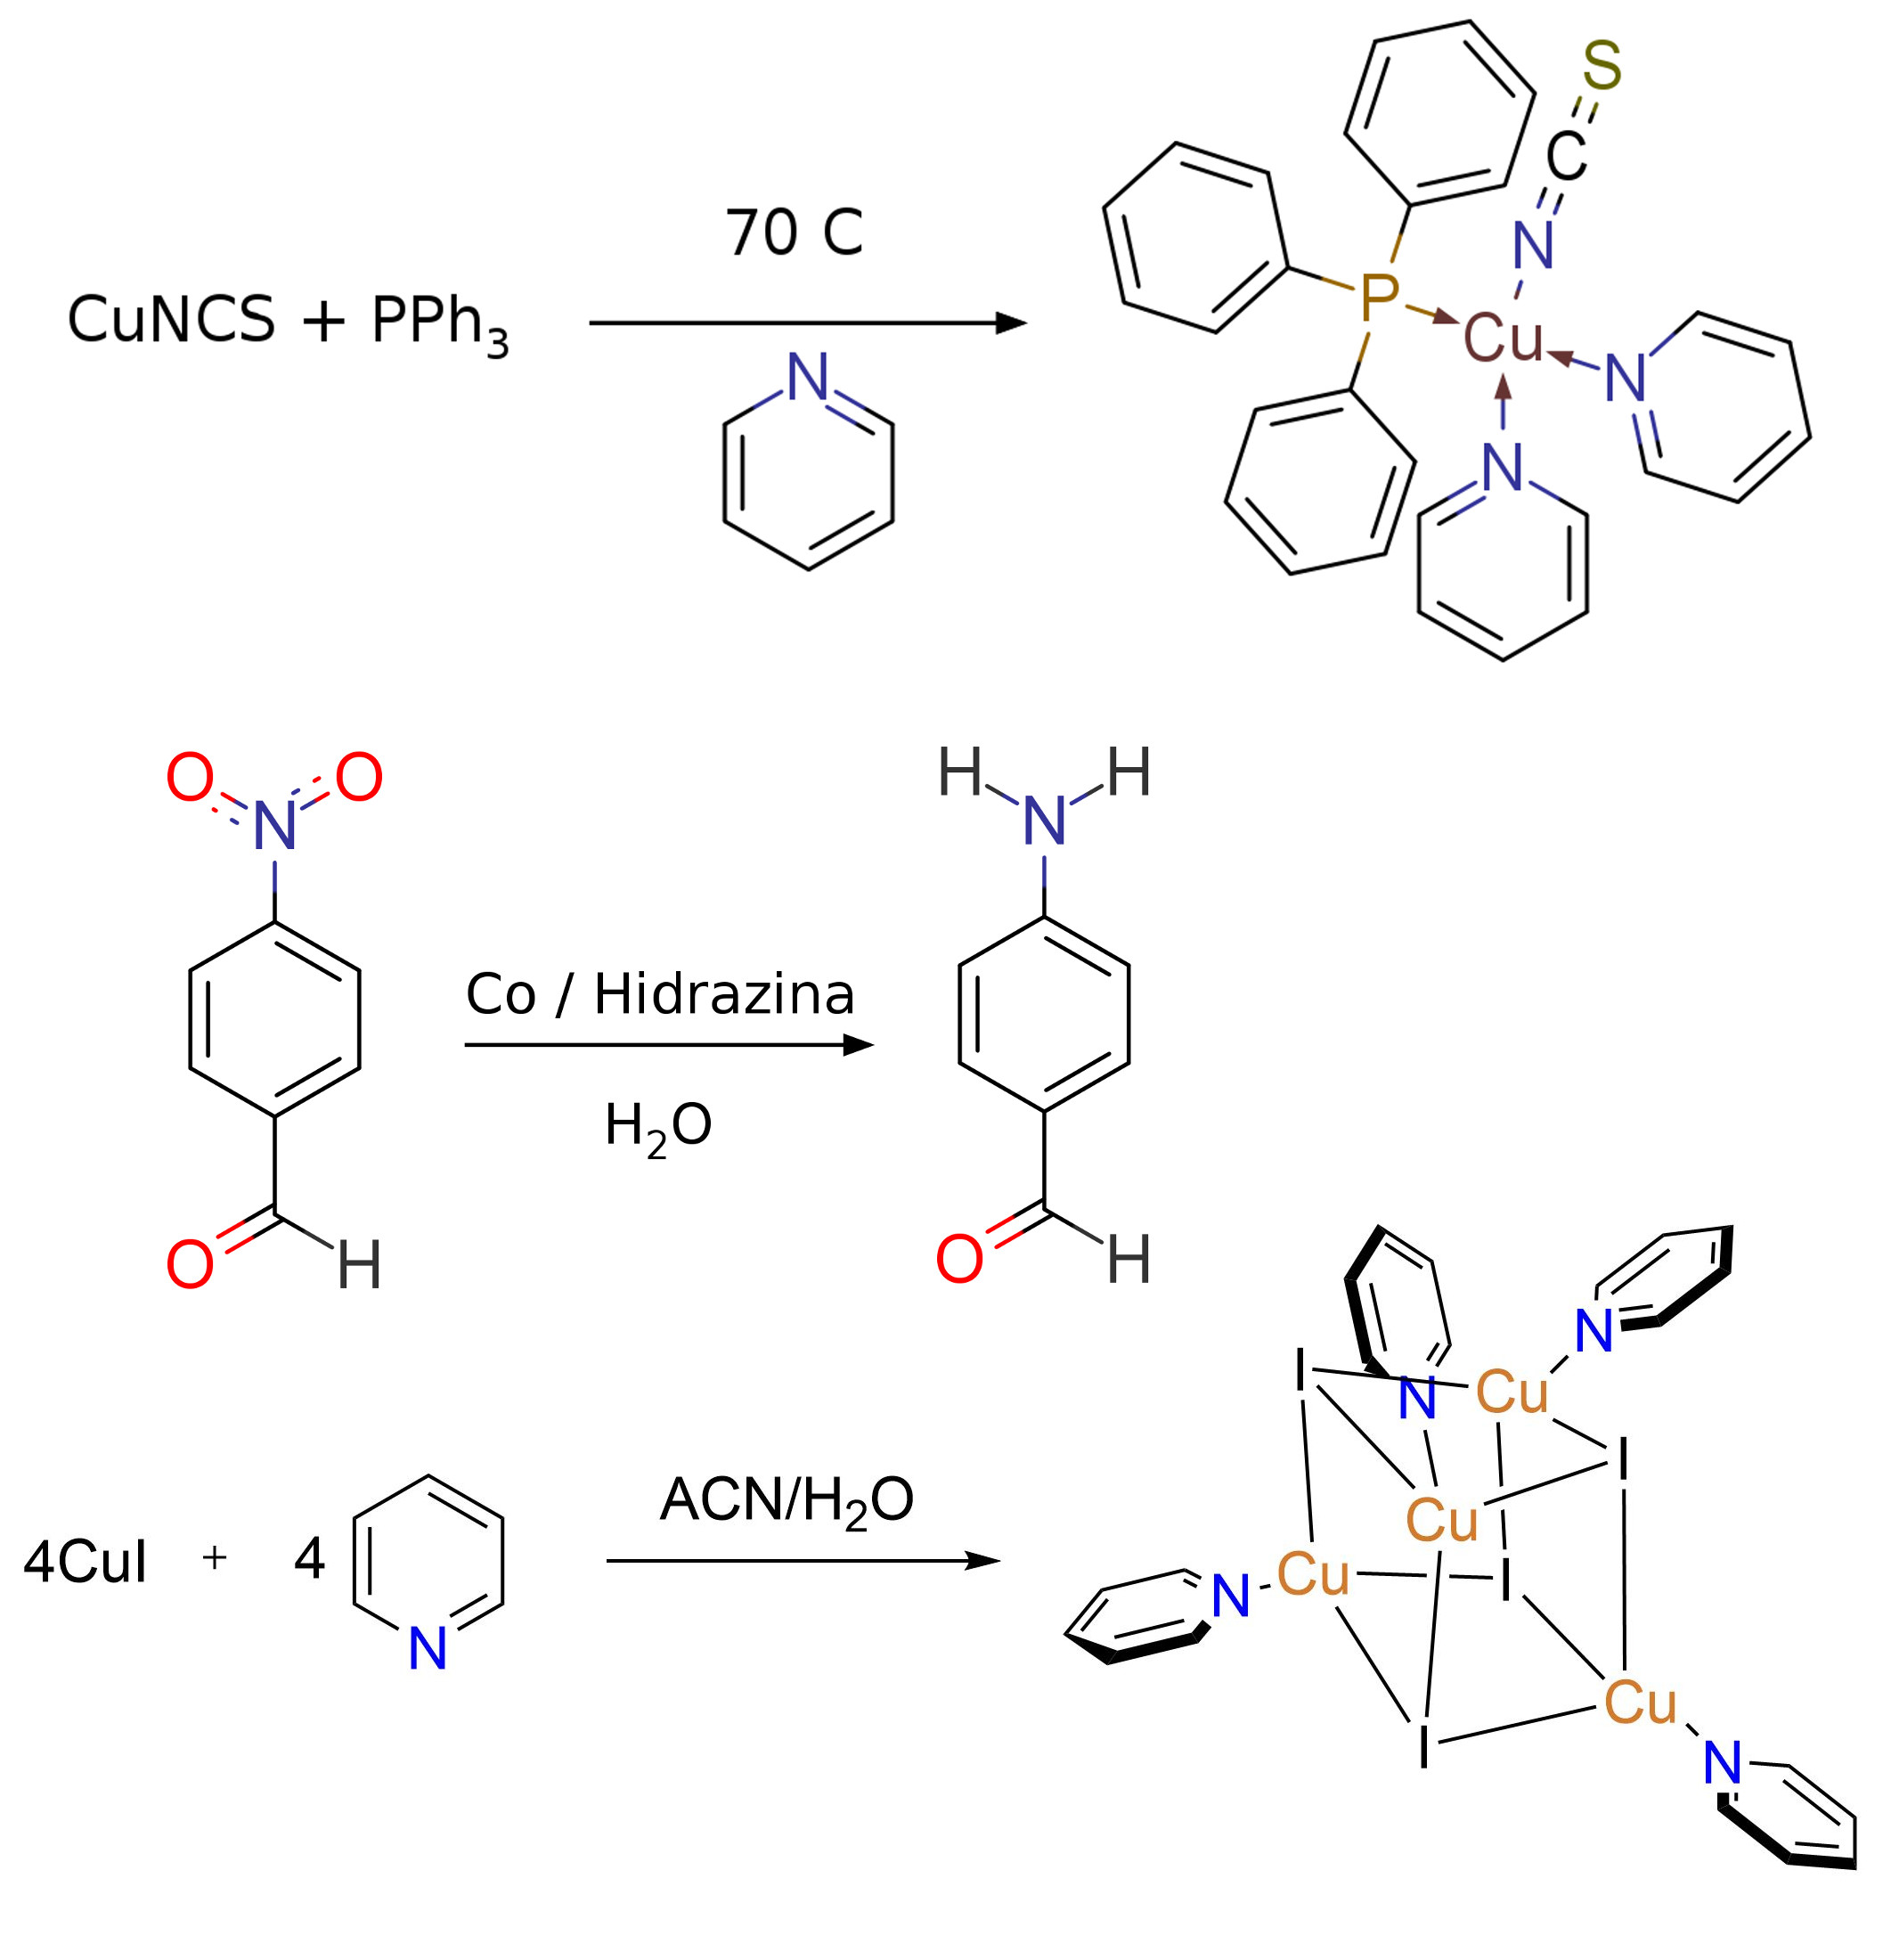
\includegraphics[width=0.65\linewidth]{Structures/Complete.jpg}
	\end{wrapfigure}
	Tres compuestos inorg\'anicos representativos de la triboluminiscencia, nanopart\'iculas y termocromismo son sintetizados a partir de sales de metales de transici\'on. Para triboliminiscencia y termocromismo se usa sulfato de cobre como fuente de cobre (II), y las nanopart\'iculas se obtienen a partir de cloruro de cobalto (II) hexahidratado. Los rendimientos obtenidos corresponden con 75 \% para el complejo tribolumniscente \ce{[Cu(NCS)(py)2(PPh3)]}, 89 \% para la formaci\'on de nanopart\'iculas de Co y 77 \% para el cluster termocr\'omico \ce{Cu4(py)4I4}. El presente cuenta con una breve introducci\'on a los fen\'omenos f\'isicos y qu\'imicos involucrados en la triboluminiscencia y termocrom\'ia, las reacciones involucradas son discutidas, y el mecanismo de reacci\'on de la reducci\'on con nanopart\'iculas es presentado. \\
}

%----------------------------------------------------------------------------------------

\begin{document}

\flushbottom % Makes all text pages the same height

\maketitle % Print the title and abstract box

%\tableofcontents % Print the contents section

\thispagestyle{empty} % Removes page numbering from the first page



%----------------------------------------------------------------------------------------
%	ARTICLE CONTENTS
%----------------------------------------------------------------------------------------

\section*{Introducci\'on} % The \section*{} command stops section numbering

La triboluminiscencia es un fen\'omeno electromagn\'etico donde se obtiene emisi\'on de luz producto de estr\'es mec\'anico sobre un material. El fen\'omeno fue descubierto en 1605, sin embargo a pesar de ser estudiado por varios siglos y en procesos tan variados como el rompimiento de los cristales de azucar, la cristalizaci\'on de algunas sustancias \cite{weiser_1917}, hasta la emisi\'on inducida por laser de ondas de choque sobre un s\'olido \cite{tsuboi_seto_kitamura_2008}, contin\'ua siendo un enigma en la teor\'ia. Experimentalmente la luz emitida es caracterizada por espectroscop\'ia, de donde se ha podido concluir que el nitr\'ogeno se encuentra involucrado en varios de los procesos antes mencionados. La causa de la emisi\'on se relaciona con el movimiento de cargas el\'ectricas en una mol\'ecula cuyos enlaces qu\'imicos son modificados producto de una fuerza externa \cite{olawale_okoli_fontenot_hollerman_2016}.

Dependiendo de la topolog\'ia de la fuerza aplicada, la triboluminiscencia se divide en tres categor\'ias: el\'astica, pl\'astica y de fractura, siendo la \'ultima la estudiada en el presente documento. Estos procesos se caracterizan por el movimiento de cargas, en donde la carga de las superficies fracturadas es neutralizada por portadores de carga como iones \cite{olawale_okoli_fontenot_hollerman_2016}. 

Muchas de las sustancias que presentan este fen\'omeno contienen dopantes que modifican la energ\'ia de las bandas del s\'olido. Al reducirse la energ\'ia entre las bandas de conducci\'on y valencia del mismo se aumenta la probabilidad de emisi\'on, haciendo de estas sustancias materiales atractivos para detectores \cite{sage_humberstone_oswald_lloyd_bourhill_2001} \cite{olawale_okoli_fontenot_hollerman_2016}.

\pagebreak
\begin{figure}[h]
	\centering
	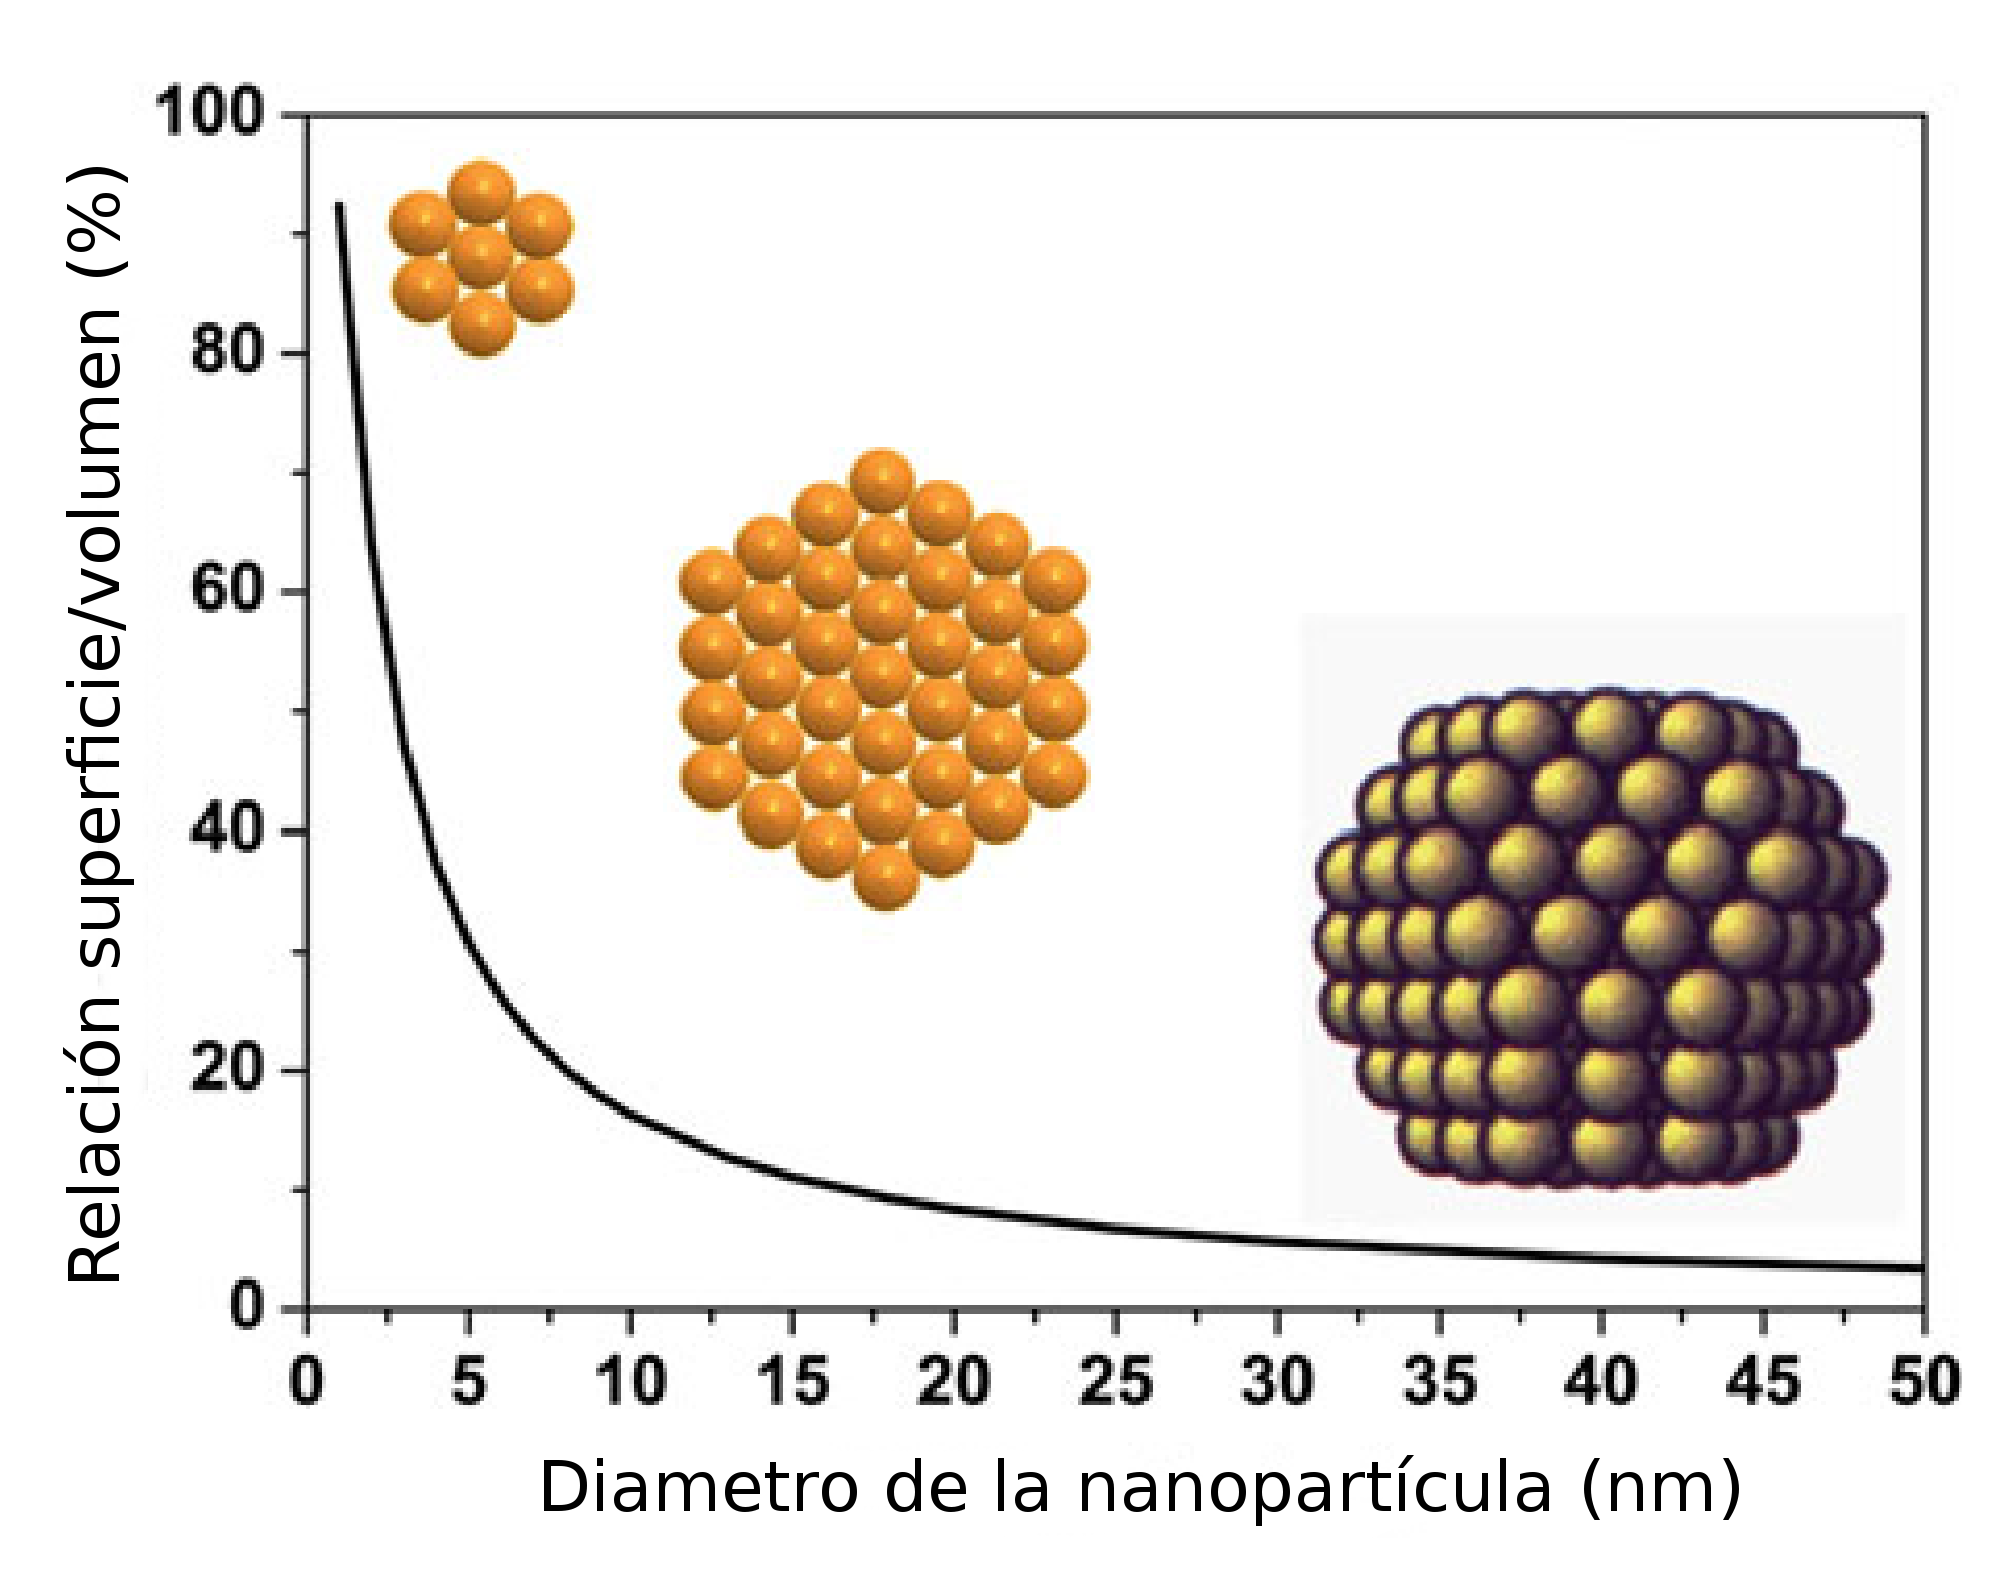
\includegraphics[width=0.8\linewidth]{Structures/nanosizes.png}
	\caption{Efecto del di\'ametro de una nanopart\'icula en la superficie de la misma. Modificado de \cite{de_mello_donega_2014}.}
	\label{fig: sizematters}
\end{figure}
Las nanopart\'iculas, por otro lado, representan un \'area de gr\'an inter\'es para la ciencia y la industria. Su popularidad se debe a que sus propiedades no dependen de la qu\'imica de sus grupos funcionales \'unicamente, si no que adem\'as presenan propiedades distintas en funci\'on del tama\~no. Lo anterior hace posible que las nanopart\'iculas sean dise\~nadas en funci\'on del tama\~no y de la qu\'imica contenida en las mismas. La dependencia de una propiedad f\'isica o qu\'imica con el tama\~no tiene dos or\'igenes en particular. En primer lugar entre menor sea el mismo la densidad de \'atomos en la superficie de la part\'icula aumenta modificando la forma como estas interact\'uan. Este efecto es considerable puesto que decae exponencialmente con el diametro de la part\'icula (\autoref{fig: sizematters}), raz\'on por la cual entre m\'as peque\~na sea, mayor ser\'a la utilidad de la misma en reacciones de cat\'alisis, por ejemplo. El segundo efecto se denomina confinamiento espacial, y se relaciona con los efectos mecanico cu\'anticos a los que se encuentra sometida la materia y que son particularmente evidentes a peque\~nas escalas \cite{de_mello_donega_2014}. Debido a que los tama\~nos de los \'atomos que constituyen una nanopart\'icula var\'ian de material en material, las propiedades relativas al confinamiento son dif\'iciles de predecir y resultan particulares a cada material.


El uso de metales de transici\'on en las hidrogenaciones se debe a la facilidad de los mismos para transferir hidr\'ogenos de una mol\'ecula a otra. En la reacci\'on de reducci\'on del 4-nitrobenzaldehido al 4-aminobenzaldehido, la fuente de hidr\'ogenos es la hidrazina. La reacci\'on catal\'itica se lleva a cabo en fase heterogenea, facilitando la separaci\'on del producto y catalizador por filtraci\'on.

Otro efecto importante en la química es el fenómeno de cromismo, en donde diversos estímulos externos son capaces de generar un cambio de color en los compuestos \cite{yang_li_zhang_zhang_2016}. Estos pueden ser clasificados como fotocromismo, electrocromismo, vapocromismo, mecanocromismo, solvatocromismo, acidocromismo y termocromismo \cite{yang_li_zhang_zhang_2016}. Este último se entiende como un cambio reversible en color de un compuesto cuando se ve sometido a cambios de temperatura. Para el caso de los compuestos inorgánicos, se conoce que esta transición se debe principalmente al cambio de la fase cristalina del complejo, a un cambio en la geometría del ligando u complejo o un cambio en el número de moléculas de solvente en la esfera de coordinación \cite{day_1968}.

Sin embargo, en algunos casos se da el fenómeno de termocromía luminiscente, en donde se genera un cambio en la emisión de fluorescencia de una molécula mediado por la temperatura \cite{parmeggiani_sacchetti_2012}. Si bien la descripción de este ha resultado ser un reto para la química inorgánica, se propone que la excitación diferencial, mediada por la temperatura, que se puede dar entre el estado basal y diferentes estados excitados de la molécula derivan en el fenómeno mencionado con anterioridad \cite{parmeggiani_sacchetti_2012}. Este fenómeno fue estudiado de manera experimental por medio de la síntesis de un cluster tetranuclear de cobre (I), piridina y yodo. 
%------------------------------------------------

\section{Resultados y Discusi\'on}
La preparaci\'on del complejo triboluminiscente de cobre se realiza en dos partes. La primera es la obtenci\'on del isotiocianato de cobre (I), lo cual se realiza a partir de tiocianato de potasio y sulfato de cobre en soluci\'on. En este punto se pueden formar dos productos, la sal de cobre (II) y la de cobre (I). La primera se produce r\'apidamente dado que no involucra cambios en los estados de oxidaci\'on de los reactivos \cite{tykodi_1991}\cite{tudela_1993}.
\begin{equation}
	\ce{Cu^{2+} (ac) + 2SCN- (ac) -> [Cu(NCS)2(s)]}
\end{equation}

A pesar que el cobre (II) es el ion m\'as estable y abundante en soluci\'on, el compuesto anterior resulta poco estable debido a que su descomposici\'on da lugar a la formaci\'on de tiocian\'ogeno \ce{(SCN)2} el cual a su vez reacciona con agua dando lugar a 3 compuestos estables: \'acido tiocianico, \'acido sulf\'urico y \'acido cianh\'idrico, donde el \'ultimo se libera en forma gaseosa, desplazando el equilibrio hacia los productos \cite{tudela_1993}.

\footnotesize
\begin{equation}
	\begin{array}{c}
		\ce{[Cu(NCS)2(s)] <=>> [Cu(NCS)(s)] + (SCN)2(ac)}\\
		\ce{3(SCN)2(ac) + 4H2O(l) <=>> 5HNCS(l) + H2SO4(l) + HCN(g)}
	\end{array}
\end{equation}
\normalsize

La reacci\'on anterior explica por qu\'e la descomposici\'on tiene lugar \'unicamente en soluci\'on y no como s\'olido seco. Adicionalmente permite entender el efecto de la temperatura como facilitadora de la conversi\'on del isotiocianato de cobre (II) al (I), dada la formaci\'on de un gas. Por otro lado, la concentraci\'on juega un papel importante en la formaci\'on del compuesto con deseado. Raz\'on por la cual el tiocianato fue agregado por goteo sobre la soluci\'on de cobre, logrando de esta forma que el producto obtenido tenga una relaci\'on 1:1.

Por otro lado es importante tener en cuenta que el ani\'on \ce{NCS-} tiene dos formas de enlazarse a otro \'atomo: por un lado con el nitr\'ogeno, por el otro con el azufre. En el caso del cobre el enlace tiene lugar con el nitr\'ogeno debido a la mayor al caracter intermedio del cobre y nitr\'ogeno como \'acidos y bases de Pearson.
\begin{scheme}
	\centering
	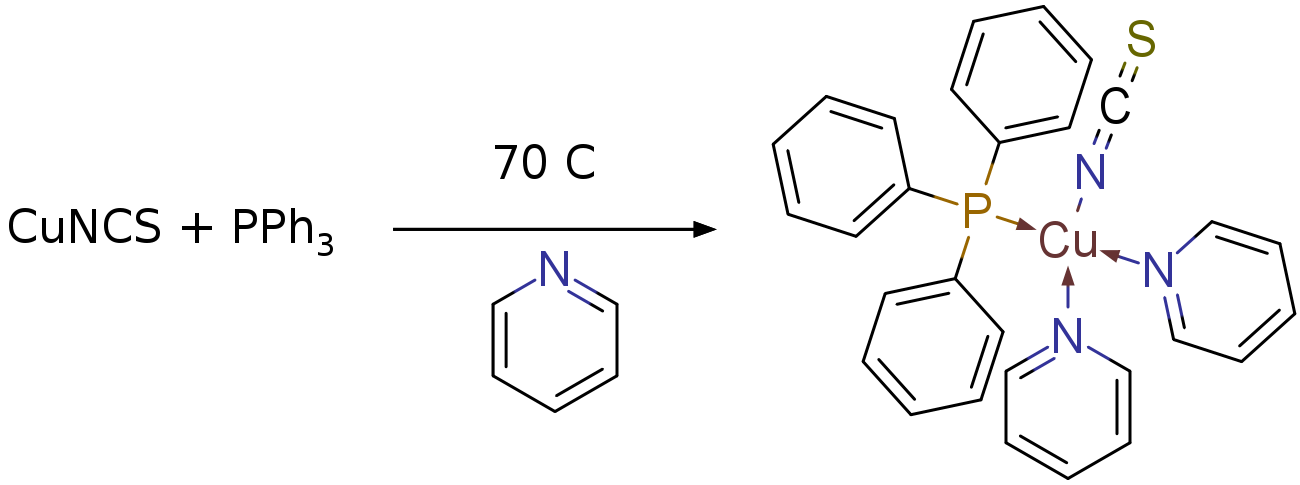
\includegraphics[width=0.8\linewidth]{Structures/tribo.png}
	\caption{Preparaci\'on del complejo \ce{[Cu(NCS)(py)2(PPh3)]}.}
\end{scheme}

La segunda reacci\'on llevada a cabo es la adici\'on al centro met\'alico de dos mol\'eculas de piridina y una de trifenilfosfina, los cuales dan lugar al \ce{[Cu(NCS)(py)2(PPh3)]}, el cual presenta una geometr\'ia tetra\'edrica distorcionada por el volumen de los ligandos. La reacci\'on es netamente coordinativa donde el f\'osforo y los nitr\'ogenos de las piridinas actuan usando sus pares libres de electrones para enlazarse con el metal.

Dado que la triboluminiscencia es de fractura es necesario el rompimiento de un enlace en el cristal. Al tener en cuenta la teor\'ia propuesta por Ahrland en 1958, en donde se clasifican los cationes seg\'un su tipo: A para los m\'as livianos y de alto estado de oxidaci\'on, y B para los m\'as pesados con estados de oxidaci\'on bajos, se observa que para el caso del cobre (I) los enlaces con f\'osforo son los m\'as estables. El enlace Cu(I)-N tiene menor tendencia a formarse y por lo tanto mayor tendencia a romperse \cite{ahrland_chatt_davies_1958}. De esta forma es posible que el enlace a romperse pueda ser el de una piridina o el de isotiocianato.

Como fue comentado en la introducci\'on, la presencia de un i\'on es necesaria para la estabilizaci\'on de las nuevas superficies \cite{olawale_okoli_fontenot_hollerman_2016}\cite{marchetti_di_nicola_pettinari_timokhin_pettinari_2012}. El \'unico ligando cuya salida implicar\'ia la formaci\'on de un cati\'on met\'alico y un ani\'on es el isotiocianato. En ese sentido el rompimiento del enlace implicar\'ia la acumulaci\'on de cargas positivas y negativas en caras opuestas. El esfuerzo mec\'anico incluye la separaci\'on de las mismas, ocasionando el surgimiento de un campo el\'ectrico entre las superficies. Los campos el\'ectricos pueden de acelerar las cargas que se encuentren bajo su efecto, los electr\'ones del ani\'on pueden alcanzar velocidades tales que ionicen el medio circundante \cite{olawale_okoli_fontenot_hollerman_2016}. Los iones del medio pueden a su vez incrementar el campo o el n\'umero de choques ionizantes, generando una reacci\'on en cadena similar a la que ocurre en una descarga el\'ectrica en un rel\'ampago, produciendo la emisi\'on de luz en los \'atomos excitados. 

En el caso de las nanopart\'iculas, la preparaci\'on se da por formaci\'on de coloides. Lo anterior se da con la reducci\'on del cobalto bajo la acci\'on del borohidrudo de sodio.
\begin{equation}
	\begin{array}{r}
		\ce{CoCl2.6H2O(ac) + 2NaBH4(ac) ->} \\
		\ce{Co(s) + H2(g) + B2H6(g) + 2NaCl(ac)}
	\end{array}	
\end{equation}

El cobalto obtenido tiene un tama\~no cercano a los 10 nm. La estabilizaci\'on de nanopart\'iculas se encuentra relacionada con interacciones electroest\'aticas en soluci\'on, raz\'on por la cual la formaci\'on de sales en la reacci\'on presenta un impacto negativo sobre las mismas, da\~nando la estructura coloidal, forzando la agregaci\'on. Para evitar la formaci\'on de enlaces \ce{Co-Co} se agrega polivinilpirrolidona en soluci\'on la cual forma una capa polim\'erica alrededor del metal, producto de las interacciones nanopart\'icula estabilizante \cite{wang_qiao_chen_wang_ding_2005}.
\begin{scheme}[h]
	\centering
	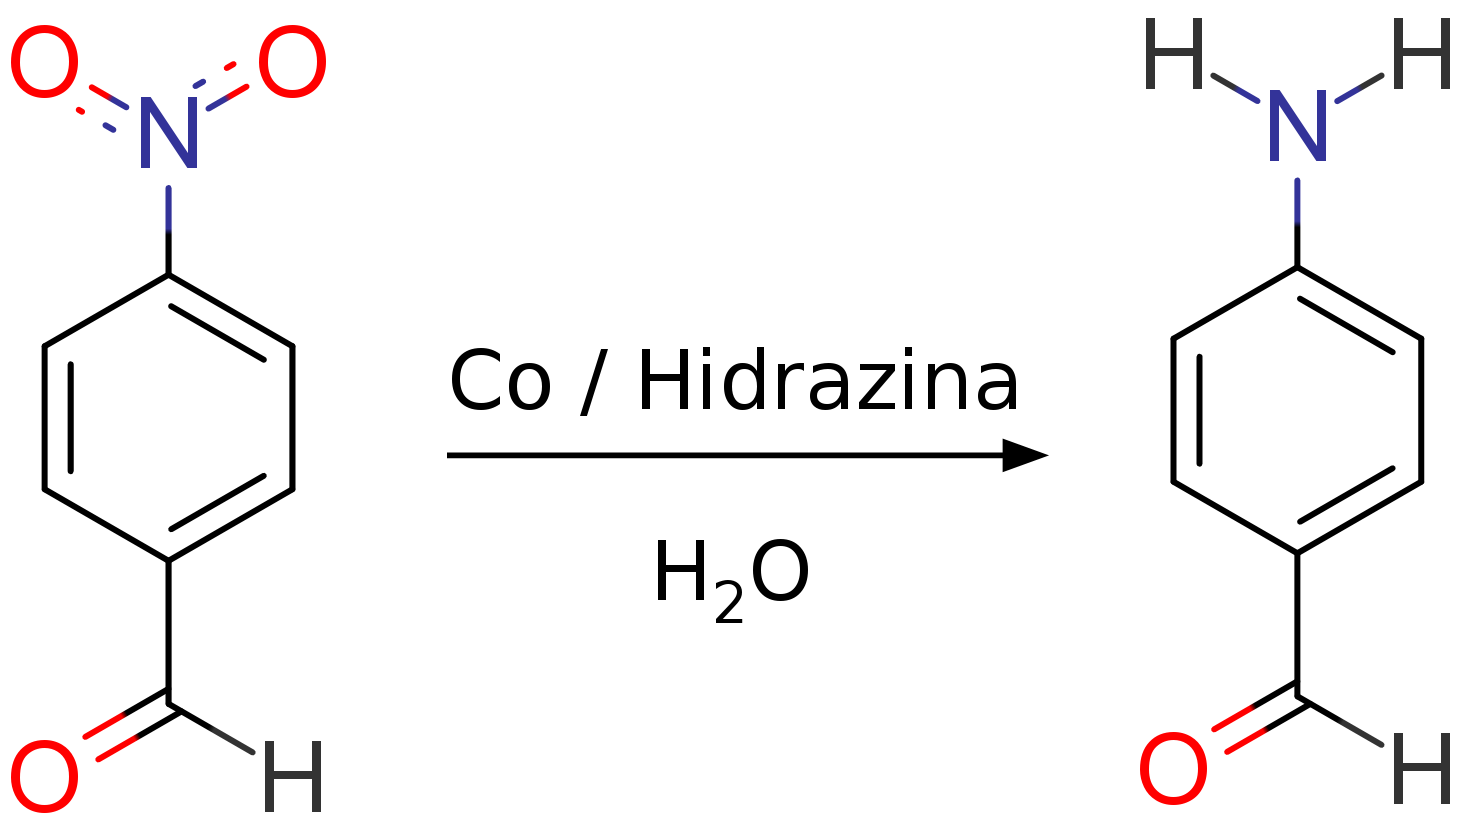
\includegraphics[width=0.5\linewidth]{Structures/reduction.png}
	\caption{Reducci\'on del grupo nitro en el $p$-nitrobenzaldeh\'ido.}
\end{scheme}

El centro met\'alico tiene la capacidad de coordinarse con los hidr\'ogenos de la hidrazina, de esta forma se genera la posibilidad de transferencia de los mismos al grupo nitro del compuesto a reducir \cite{mccleverty_meyer_2004}. El mecanismo propuesto por Rai y colaboradores presenta dos posibles rutas para la reducci\'on del grupo nitro \cite{rai_mahata_mukhopadhyay_gupta_li_nguyen_zhao_pathak_singh_2014}. La ruta directa se da por la protonaci\'on de un ox\'igeno en el grupo nitro, con posterior eliminaci\'on de agua \textit{(b)}, el producto es nuevamente hidrogenado dando lugar a un hidroxiamino \textit{(c)}. Una \'ultima reducci\'on tiene lugar con la adicci\'on de hidr\'ogenos al hidroxilo y al grupo amino, la reacci\'on da lugar a la eliminaci\'on de agua y a la formaci\'on de la amina primaria \textit{(d)}. La segunda ruta se da con la condensaci\'on de las mol\'eculas \textit{(b)} y \textit{(c)}, lo cual da lugar a un oxoazobenzeno sustituido \textit{(e)}. El ox\'igeno se elimina con la adici\'on de hidr\'ogeno dando lugar al producto en \textit{(f)} el cual puede fragmentarse en presencia de hidr\'ogeno en dos mol\'eculas de 4-aminobenzaldehido \textit{(d)} \cite{rai_mahata_mukhopadhyay_gupta_li_nguyen_zhao_pathak_singh_2014}. La selectividad hacia el grupo nitro se relaciona con la densidad de carga del mismo dado todos los \'atomos del mismo presentan pares libres que pueden atacar con facilidad a los hidr\'ogenos coordinados al metal.
\begin{scheme}[h]
	\centering
	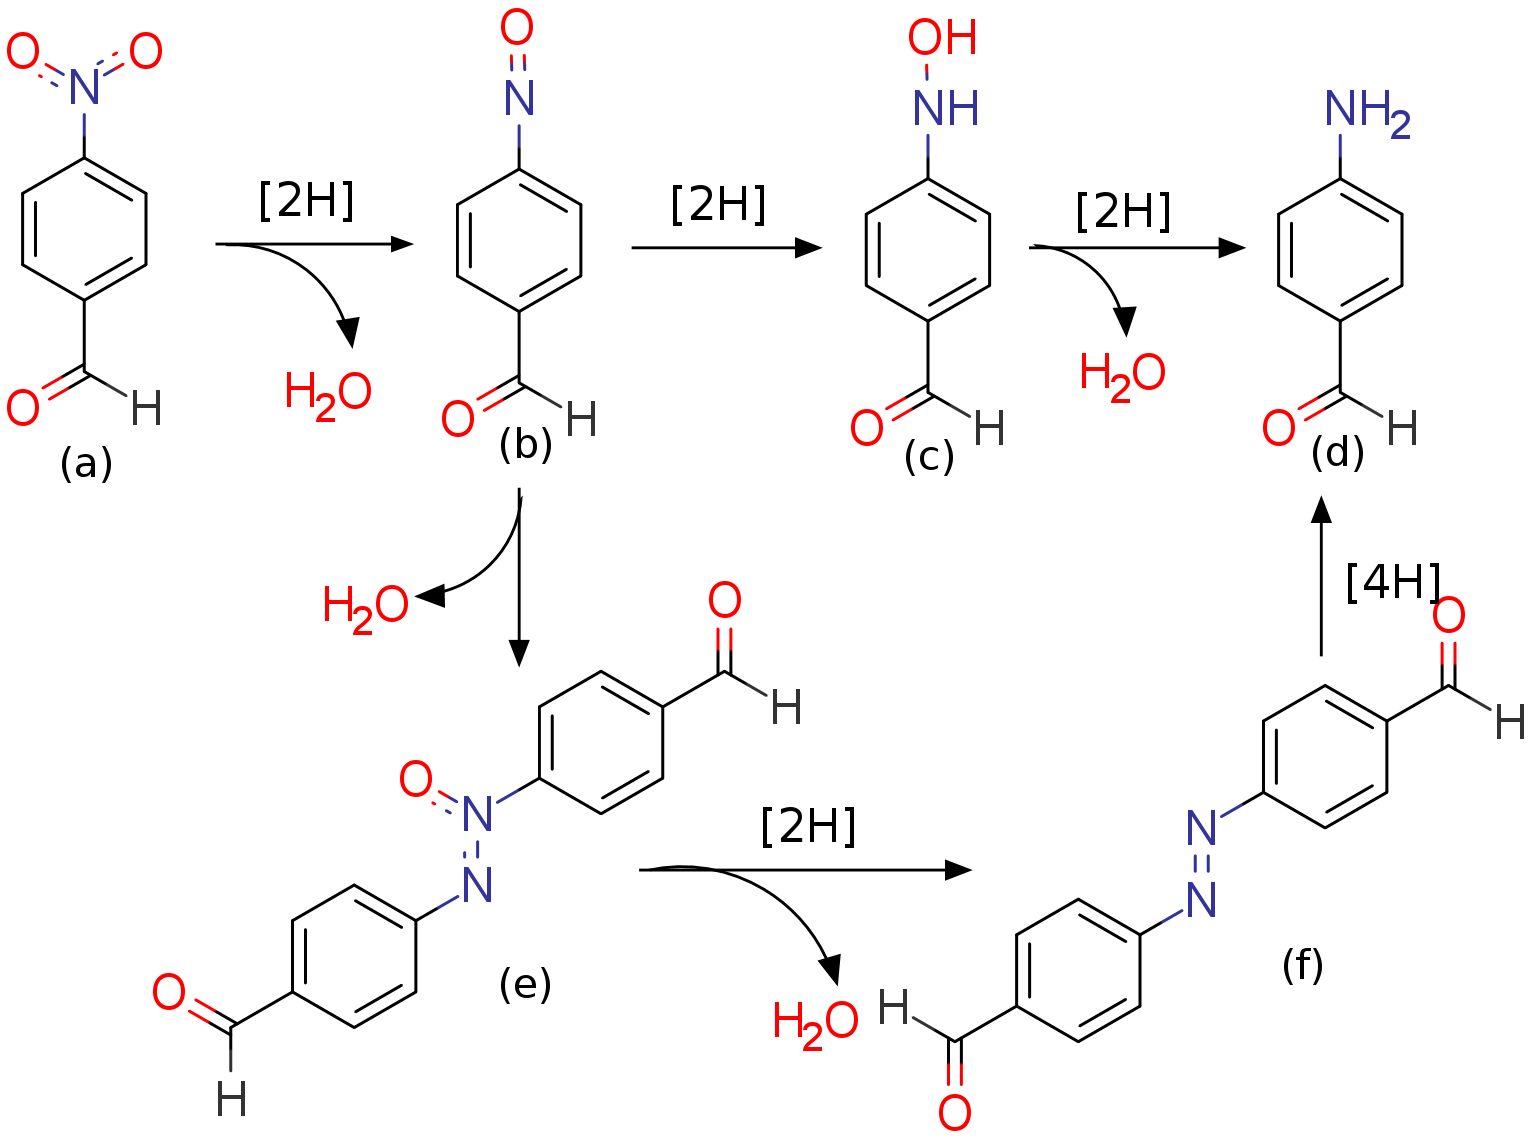
\includegraphics[width = 0.8\linewidth]{Structures/mechanism.png}
	\label{sch: mechanism}
	\caption{Mecanismo de reacci\'on propuesto para la reducci\'on de nitrocompuestos \cite{rai_mahata_mukhopadhyay_gupta_li_nguyen_zhao_pathak_singh_2014}.}
\end{scheme}

Sin embargo, la catálisis realizada experimentalmente no mostró la selectividad esperada. En el el 1H-RMN tomado del producto tras los procesos de centrifugación efectuados (\autoref{fig: RMN}), se pudo observar un alto grado de impureza en el sólido recuperado. Fue posible identificar los picos asociados al producto ($^1$H NMR (400 MHz, DMSO) $\delta$ 8.17 (d, $J$ = 8.6 Hz, 1H), 7.68 (d, $J$ = 8.5 Hz, 1H), 7.56 (s, 1H)), observándose más a campo bajo los protones aromáticos correspondientes a las posiciones \textit{orto} del aldeh\'ido, siguiendo hacia campo alto los protones en \textit{meta} del mismo, seguido de los protones de la amina. No se pudo identificar el protón del aldehído.

Sin embargo, se observan otras señales, de las cuales algunas se identificaron como producto de partida (Esperando que estas se encontraran más a campo bajo por el efecto extractor de carga del \ce{NO2} sobre el anillo aromático) y otras no fueron identificadas, por lo cual se asocian directamente a productos secundarios generados en la reacción.

Teniendo en consideración lo anterior, se puede decir que la catálisis no mostró la selectividad esperada, haciendo necesario pasos adicionales de purificación del producto. Sin embargo, no se puede desconocer que si se observó producto, por lo cual se confirma que la reacción si se efectuó. 

De manera experimental, la síntesis del cluster termocrómico \ce{Cu4(py)4I4} pudo ser comprobada por medio del fenómeno de termocromía fluorescente observado de manera experimental \autoref{fig: thermo}.
\begin{figure}[h]
	\centering
	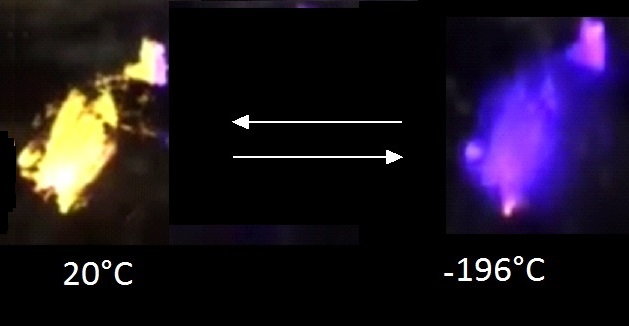
\includegraphics[width=0.7\linewidth]{Structures/thermo.jpg}
	\caption{Colores observados bajo longitud de onda de 352 nm a 20$^\circ$C y -196$^\circ$C para el cluster sintetizado.}
	\label{fig: thermo}
\end{figure} 

\pagebreak
La síntesis de este cluster se logró realzar de manera eficiente experimentalmente. Esta se efectuó en dos pasos (i) Síntesis de CuI (2) Síntesis del cluster termocrómoco. 
Para la primera etapa de reación, se partió de sulfato de cobre(II), el cual fue disuelto en agua y ligeramente acidificado con una solución de sulfito de cobre sobre ácido sulfurico, y posteriormente  hecho reaccionar con yoduro de potasio (\autoref{eq: thermo}).
\begin{equation}\label{eq: thermo}
	\begin{matrix}
		\ce{2CuSO4(ac) + 2KI(ac) + SO2(ac) + 2H2O(l) ->} \\
		\ce{2CuI(s) + 2H2SO4(ac) + K2SO4(ac)}
	\end{matrix}
\end{equation}

De esta etapa es importante resaltar que se presentó un problema con la consistencia de la sal sintetizada, puesto que esta al estar humeda presenta un grado de viscosidad que hace dificil su manejo posterior a la filtración. Por este motivo si bien en la litaratura se menciona que no es necesario que este producto sea secado previo a la etapa dos de síntesis \cite{parmeggiani_sacchetti_2012}, experimentalmente se recomienda secar la sal para su posterior manejo. En cuanto las etapas que llevaron a la síntesis de la misma,  se destaca el rol de la solución ácida de sulfito, puesto que esta es necesaria para efectuar la redución que deriva en la síntesis de una sal de Cu(I) a partir de una sal comenrcial de Cu(II). 

En cuanto la segunda etapa de sintesis, (\autoref{sch: thermo}) es importante resaltar que para evitar la oxidación del Cu(I) en el medio de reacción, es necesaria la adición del yoduro de potasio, puesto que en el medio ácido para la reacción el KI es capaz de oxidarse lentamente \cite{delury_1902}.
\begin{scheme}[h]
	\centering
	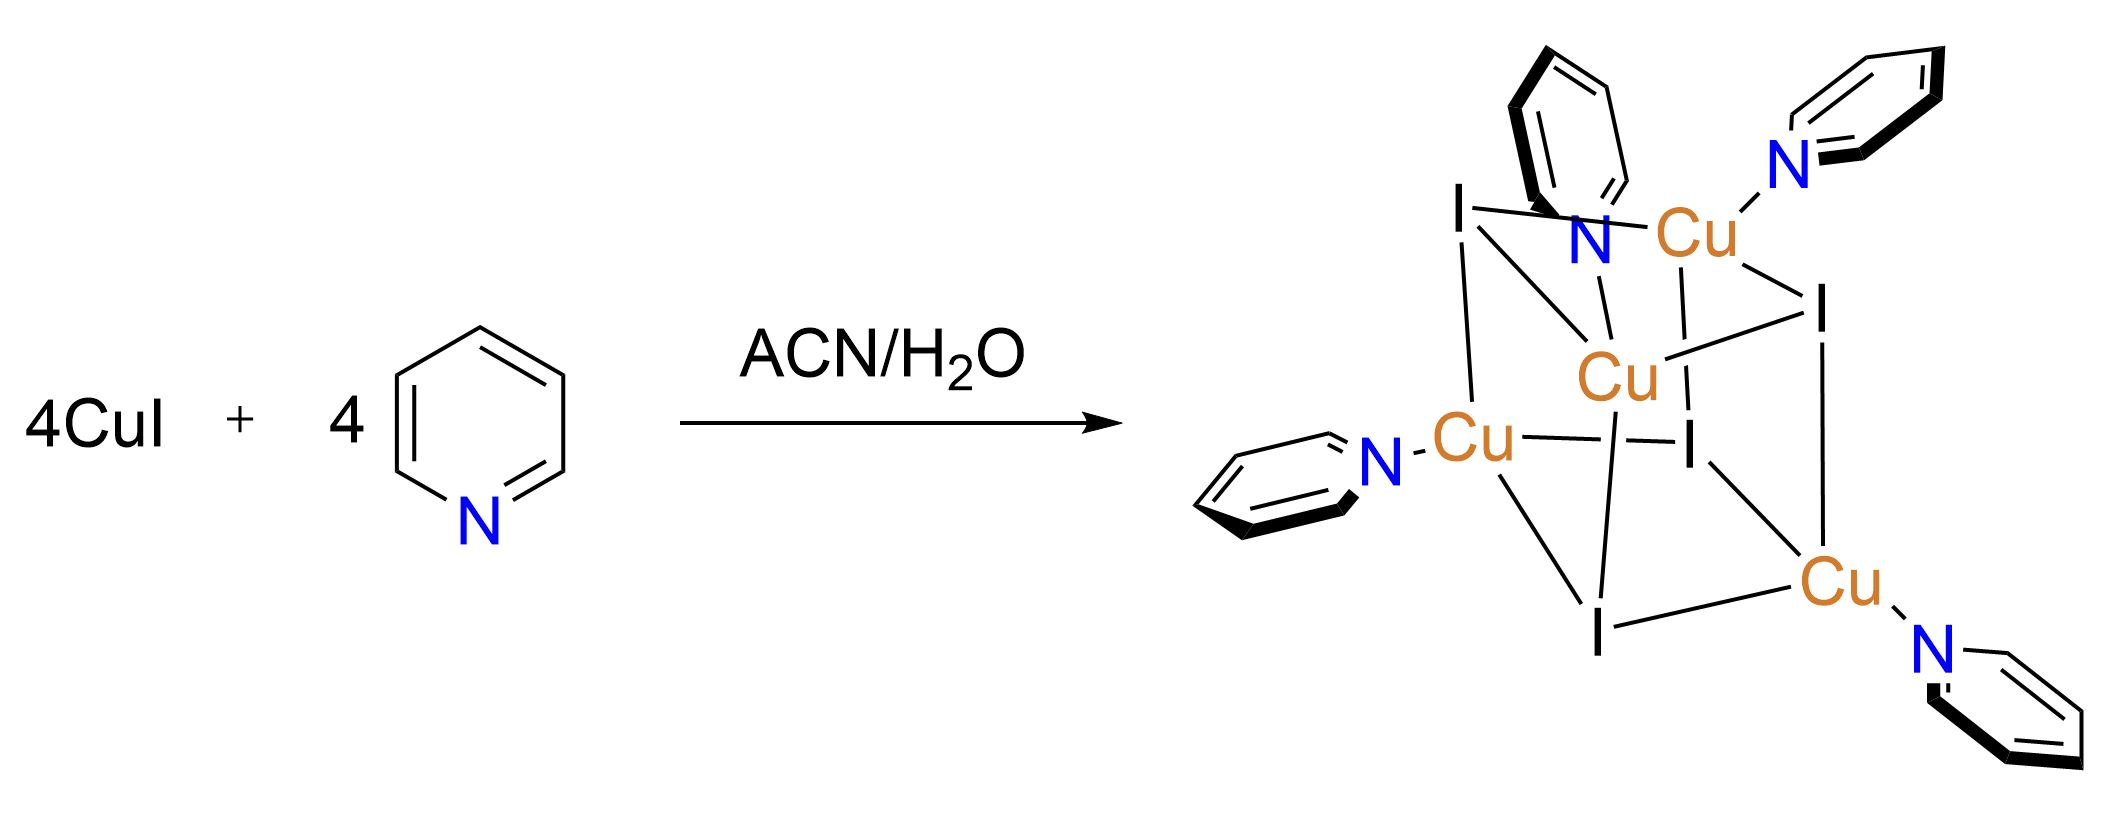
\includegraphics[width=0.8\linewidth]{Structures/thermo_scheme.JPG}
	\caption{Etapa 2 de reacción. Síntesis del cluster termocrómico.}
	\label{sch: thermo}
\end{scheme}

En cuanto al fenómeno observado, se propone en la literatura que este se debe al cambio en las  intensidades relativas de las dos bandas de absorción de este complejo. Se reporte que la banda de absorción más energética es la asociada al estado triplete excitado de la banda de transferencia de carga haluro-ligando (alrededor de 450 nm), y la banda menos energética asociada a al estado triplete excitado de la banda de transferencia de carga haluro-metal con una combinación de transiciones d-s presentes en el cluster \cite{parmeggiani_sacchetti_2012}. Según estudios realizados, se conoce que a temperatura ambiente, la banda menos energética es predominante en el medio, mientras que a bajas temperaturas, es la otra banda la de mayor intensidad \cite{yang_li_zhang_zhang_2016}\cite{parmeggiani_sacchetti_2012}\cite{kitagawa_ozawa_toriumi_2010}.

Teniendo lo anterior en consideración se puede pensar que la migración electrónica asociada a uno u otro estado excitado se influenciado directamente por la temperatura. Para el caso de la excitación electrónica al orbital vacío en fase en el espacio atómico s/p en el centro del complejo (Banda de alta energía), se conoce que el centro metálico se ve contraído mientras que el tetraedro del haluro expandido, generando una deformación en la estructura tipo cubano del cluster \cite{kitagawa_ozawa_toriumi_2010}. Al bajar la temperatura, la contracción del centro metálico puede afectar el empaquetamiento del cluster, generando una deformación del mismo mediado por la presión externa generado por las piridinas. Esto deriva en que a bajas temperaturas, banda asociada a la transferencia de carga entre la piridina y el haluro se vea menos favorecida en relación a la banda asociada a la estructura del cluster \cite{kitagawa_ozawa_toriumi_2010}. Ahora bien en términos de orbitales se puede decir que a una baja temperatura, la misma deformación de la celda cristalina favorece la interacción entre el Cu y el I, generando así el efecto previamente mencionado.

Por último, es importante mencionar que el acoplamiento spin-orbital que se da entre los enlaces del metal y el haluro de manera general se ve favorecido a bajas temperaturas, lo que permite a su vez que el estado triplete excitado tenga una menor energía, favoreciendo así el solapamiento con el estado singlete excitado, lo que permite que se dé el aumento en el fenómeno de fluorescencia \cite{kitagawa_ozawa_toriumi_2010}.

\section{Conclusiones}
Por un lado, se logró la síntesis del \ce{[Cu(NSC)(py)2(PPh3)]}, de la misma manera que se pudo corroborar experimentalmente la triboluminicencia del mismo. Se destaca la importancia en el orden de adición de los reactivos para la primera etapa de síntesis, en donde la forma más eficiente para la sintesis del CuNCS fue la adición gota a gota de la solución de tiocianato sobre la solución de cobre.

Por otro lados, se logró la síntesis de nanopartículas de cobalto, de la misma manera que se efectuó la síntesis de la 4-aminobenzaldehido partir del 4-nitrobenzaldehido. Se concluye a raiz del sólido recuperado, que esta síntesis no de efectuó de manera selectiva.

Por último, se efectuó la síntesis del \ce{Cu4I4(py)4} y se confirmó el fenómeno de termocromía luminiscente del mismo. Se puede decir que esta síntesis no presentó mayores complicaciones, sin embargo se recomienda secar la sal formada en la primera etapa de síntesis para la mejor manipulación de la misma. 


\newpage
\section{Secci\'on experimental}
\subsection{S\'intesis de \ce{[Cu(NCS)(py)2(PPh3)]}}
La preparaci\'on de las sales se realiza usando dos soluciones 0.25 M (3.1 eq) de tiocianato de potasio y sulfato de cobre anhidro. Sobre un bal\'on con 25 mL de la soluci\'on de sulfato de cobre son adicionados 25 mL de la soluci\'on de tiocianato por goteo. La reacci\'on se calienta y agita por media hora, posteriormente se filtra el producto al vac\'io. Una mezcla con 0.2526 g (1.0 eq) de tiocianato de cobre (I) y 0.5300 g (1.0 eq) de trifenilfosfina se disuelve en 10 mL de piridina. La reacci\'on se lleva a cabo en reflujo por 3 horas.

\subsection{Reducci\'on con nanopart\'iculas}
Una soluci\'on tetrahidroborato de sodio (\ce{NaBH4}) se prepara con la disoluci\'on de 0.080 g del mismo (5.0 eq) en 10 mL de agua. Se prepara una segunda soluci\'on con 0.259 g de polivinilpirrolidina junto con 0.100 g de cloruro de cobalto hexahidratado (1.0 eq) en 10 mL de agua. La soluci\'on de \ce{NaBH4} se adiciona por goteo en presencia de ultrasonido. El producto obtenido se separa en dos mitades, una de las cuales se hace reaccionar con 0.1504 g de \textit{p}-nitrobenzaldehido (2.4 eq) y 0.2 mL de hidracina hidratada. La reacci\'on tiene una duraci\'on de 90 minutos del inicio de la reacci\'on. La reacci\'on se sigue por cromatograf\'ia de placa delgada, usando diclorometano. La separaci\'on se da por centrifugaci\'on, extracci\'on l\'iquido - l\'iquido con acetonitrilo y posterior evaporaci\'on a presi\'on reducida.

\subsection{S\'intesis de un cluster termocr\'omico}
Tres soluciones acuosas con vol\'umenes 15 mL, 30 mL y 10 mL son preparadas. La primera contiene 1.6205 g de sulfato de cobre pentahidratado (34.4 eq), la segunda 0.5000 g de sulfito de sodio (21.0 eq) y la tercera 1.0800 g de yoduro de potasio (34.5 eq). Sobre la segunda soluci\'on se adiciona \'acido sulf\'urico concentrado y se mezcla con la primera. Una vez disueltos los s\'olidos se adiciona la \'ultima soluci\'on a la mezcla. El yoduro de cobre obtenido se agrega a una soluci\'on 0.52 mL de piridina (34.2 eq) y 5 mL de acetonitrilo (508.7 eq), sobre la misma se adicionan 0.7726 g de yoduro de potasio (24.7 eq) y 0.0332 g de \'acido asc\'orbico (1.0 eq). La soluci\'on se agita por 15 minutos, posterior a los cuales se adicionan 25 mL de agua. El producto se filtra al vac\'io.  

%----------------------------------------------------------------------------------------
%	REFERENCE LIST
%----------------------------------------------------------------------------------------
\phantomsection
\bibliography{informe}
\bibliographystyle{unsrt}

%----------------------------------------------------------------------------------------
\newpage
\onecolumn
\section{Informaci\'on suplementaria}
\begin{figure}[h]
	\centering
	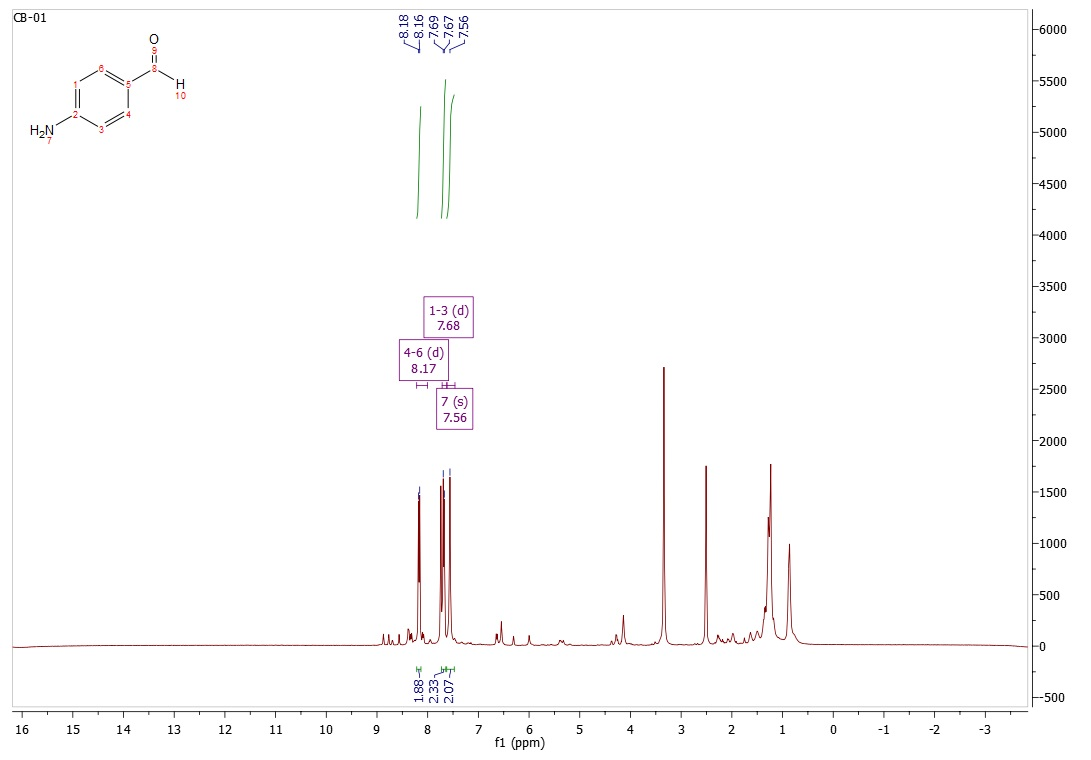
\includegraphics[width=\linewidth]{Structures/RMN.jpg}
	\caption{Resonancia magn\'etica nuclear de la muestra obtenida luego de la reducci\'on de $p$-nitrobenzaldeh\'ido con nanopart\'iculas de cobalto.}
	\label{fig: RMN}
\end{figure}
\end{document}